\begin{center}

\rule{\textwidth}{1pt}
\rule{\textwidth-1cm}{0.4pt}\\
\vspace{0.3cm}
\textsc{\HUGE F-spexet 2022}\\
%\vspace{0.025\textheight}
\rule{0.3\textwidth}{0.4pt}\\
\vspace{0.025\textheight}
\textsc{\HUGE Tillbaka till dåtiden}\\
\vspace{0.2cm}
\textsc{\large eller}\\
\vspace{0.005\textheight}
\textit{\LARGE Einsteins äventyr i rumtiden}\\
\vspace{0.010\textheight}
\textsc{\normalsize eller}\\
\vspace{0.005\textheight}
\textit{\Large Albert the Explorer}\\
\vspace{0.0075\textheight}
\textsc{\small eller}\\
\vspace{0.0025\textheight}
\textit{\large Konsten att bibehålla en konstant rumtid}\\
\vspace{0.005\textheight}
\textsc{\footnotesize eller}\\
\textit{\normalsize Cyberpunk 2052}\\
\vspace{0.0025\textheight}
\textsc{\tiny eller}\\
\textit{\small Frågan är inte \emph{var} vi parkerade tidsmaskinen, utan \emph{när} vi parkerade tidsmaskinen}\\
\hrulefill\\
\vspace{\fill}
\parbox[c][][c]{0.45\textwidth}{\centering 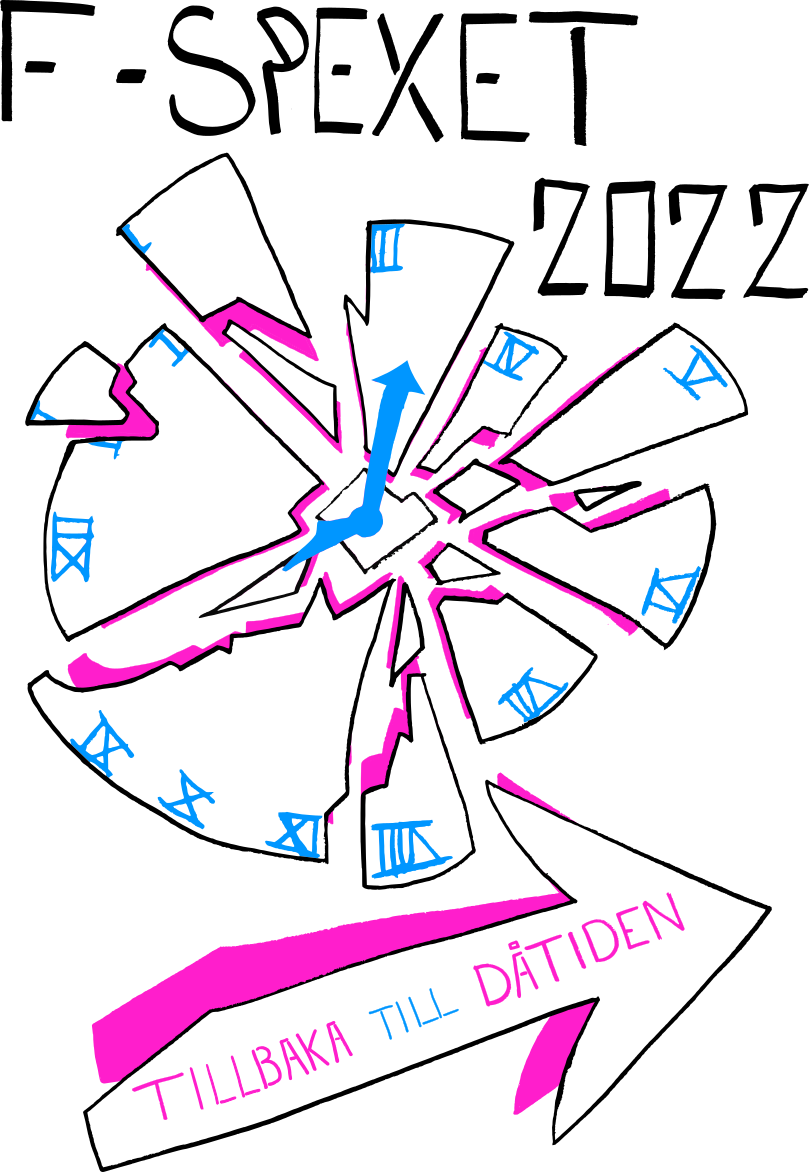
\includegraphics[width=0.35\textwidth]{Bilder/TidigareSpexloggor/2022Datiden.png}}
\parbox[c][][c]{0.45\textwidth}{\centering 
\includegraphics[width=0.33\textwidth]{Bilder/Loggor/Spexloggaoifylld3.png} \\\vspace{0.2cm}

\includegraphics[width=0.27\textwidth]{Bilder/Loggor/studieframjandet_samarbete.jpg}}


% \adjincludegraphics[width=0.3\textwidth]{Bilder/Loggor/Spexloggaoifylld3.png}
% \hspace{0.03\textwidth}
% \adjincludegraphics[width=0.3\textwidth]{Bilder/TidigareSpexloggor/2022Datiden.png}
% \hspace{0.03\textwidth}
% \adjincludegraphics[width=0.3\textwidth]{Bilder/Loggor/studieframjandet_samarbete.jpg}
\rule{\textwidth}{1pt}
\end{center}

\newpage

\vspace*{\fill}
\begingroup
\raggedright{
\huge{“En lycklig man är för nöjd med nuet för att vistas för mycket i framtiden” \\}
}
\endgroup
\begingroup
\begin{centering}
\huge{\ \\
\emph{\hspace{65mm} -- Albert Einstein}}
\end{centering}
\endgroup
\vspace*{\fill}
\newpage
%\null